\documentclass[tikz]{standalone}
\usepackage{amsmath}
\usepackage{pgfplots}
\usetikzlibrary{backgrounds}
\pgfplotsset{compat=newest}

\begin{document}
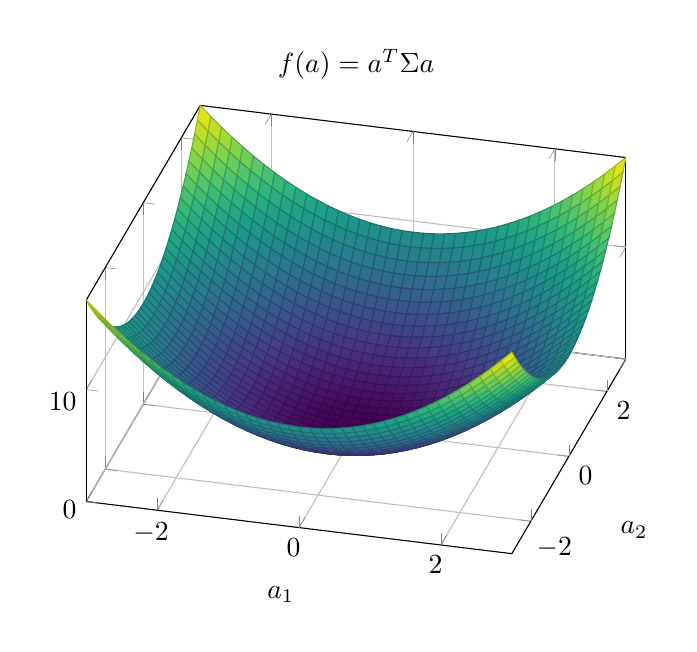
\begin{tikzpicture}[background rectangle/.style={fill=white}, show background rectangle,]

\begin{axis}[
    colormap/viridis,
    view={15}{45},
    enlargelimits=false,
    grid=major,
    domain=-3:3,
    y domain=-3:3,
    samples=41,
    zmin=0,
    zmax=18,  % Adjust as needed
    xlabel=$a_1$,
    ylabel=$a_2$,
    title={$f(a) = a^T \Sigma a$},
]
\addplot3 [surf] { x^2 + y^2 } ;  % Parabola function
\end{axis}
\end{tikzpicture}
\end{document}
